\section{Our Model}
\begin{wrapfigure}{r}{.5\textwidth}
  \begin{center}
    \resizebox {.5\columnwidth} {!} {
      \begin{tikzpicture}
        \genealogytree[template=signpost]{
          child{
            g{Agent}
            child{
              g{World Agent}
              child{
                g{Users}
              }
              c{Sources}
            }
            % c[phantom=5em]{aaaaaaa}
            child{
              g{Sky Agent}
              child{
                g{Agent Manager}
                child{
                  g{Agent Manager\\Message Scheduler\\AMMS}
                }
                c{Agent Manager\\Connection Scheduler\\AMCS}
                c{Agent Manager\\Memory Scheduler\\AMME}
              }
            } 
          }
        }
      \end{tikzpicture}
    }
  \end{center}
  \caption{Hierarchy of classes}
  \label{fig:hierarchy}
\end{wrapfigure}
We use the SLAPP3 platform for agent simulation: this environment provides agent
based protocol in Python 3.
We implemented a hierarchy of agents to manage the different abilities of
each breed.
\\
The class \textit{Agent} is the common and oldest ancestor,
it has to be so because of SLAPP's structure.\\
Next we have two main classes, defining the main branches,
one for the 'real' agents,\textit{WorldAgent}, and another for
the abstract ones, \textit{SkyAgent}.
The first of the two can represent living creatures or tangible objects;
the second can be thought as an external agent, living outside the world.\\
Of all the classes implemented only five breeds are produced during
the execution of the program.
This structure allows easy changes and possible future implementations
of the code.
\subsection{WorldAgent}
From this branch sprouts two leafs of the tree: the classes \textit{User}
and \textit{Source}.
The common variables passed by \textit{WorldAgent} are
the vector of mind state and the database of news, used both for remember
and as a storage. The common members are trivial.
Specifically talking, the state of mind is a normalized vector of a
specified dimension in the variable \texttt{dim} inside
\textit{commonVar.py}.
\subsubsection{Source}
Sources have a peaked mind state initializated during construction.
The initialization is binary with a number of non zero values from one to three:
after that, noise is added and the vector is normalized.
Each \textit{Source} has a method, \textit{generateNews}, that can produce
a news with a vector of topics inside 'near' the state of the source.
We use near, talking of states, like we talk of geometrical vectors: we will
measure the mind distance with scalar products of these vectors.
\subsubsection{User}
The main class of the program is \textit{User}.
This object contains all the functions to act indipendently in the world.
We will provide a description of the most important ones.
As mentioned before, a user can compute distance, with the homonymous
function, between mind states and between a mind state and a
topic inside news. He can make an opinion of what he sees.
He has a bunch of function to detect who are his neighbours, if they
are sources or users, and if there are only sources around him.
A user can also decide to become active or inactive using internal rules.
He can create or remove an edge between another agent.
Other important actions of users are the way they can diffuse:
\textit{activeDiffusion} and \textit{passiveDiffusion} are the
two functions used to spread news. We will talk about them later.
Finally an agent can choose how and who manage edges with using
\textit{createEdge} and \textit{deleteEdge}.
\subsection{SkyAgent and AgentManager}
\textit{SkyAgent} has an only child: \textit{AgentManager}.
He is responsible of all the logs and the managing of the agent themselves.
Other skyagents can be implemented but we do not need them for now.
\subsubsection{The Schedulers}
There are three leafs out of the \textit{AgentManager's} branch:
\textit{MessageScheduler}, \textit{ConnectionScheduler} and
\textit{MemoryScheduler}. They will be called with their initials,
respectively \textit{AMMS}, \textit{AMCS} and \textit{AMME}.
\begin{itemize}
\item[\textit{AMMS}] This scheduler registers all the spreading during the
  execution. It focuses on the news and registers their creation and
  diffusion, also distinguishing the passive and the active diffusion.
\item[\textit{AMCS}] With the connection scheduler we can take note of
  all operations correlated to edges: creation, destruction and weight
  change will be registerd in a log file.
\item[\textit{AMME}] This is unlike the other logs. The call of this log is
  not from an user but from the observer. For every cycle of the program
  this scheduler will print the database of each agent and the activation
  state of anyone.
\end{itemize}
\begin{figure}[htpb]
  \centering
  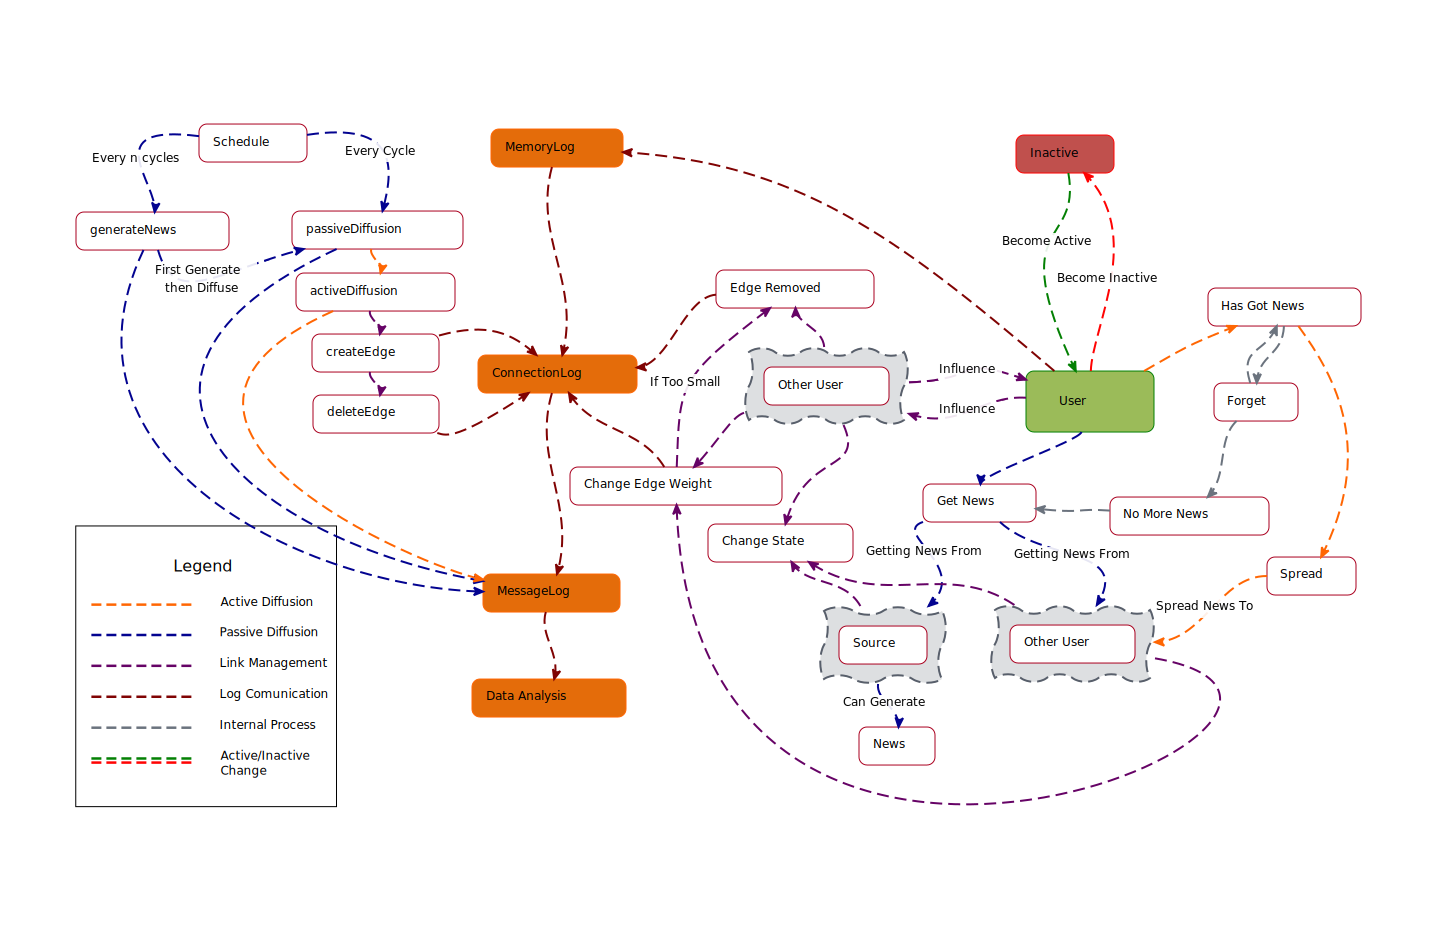
\includegraphics[width=\columnwidth]{mindMap.pdf}
  \label{fig:mindmap}
  \caption{Mind map of the model}
\end{figure}

The agents involved are structured in a hierarchy. 
Schedule: modo per programmare le varie azioni, in ordine temporale esplicitamente dato d noi.  Le azioni possono essere performate con una certa probabilità... removelinks...
Si interfaccia alle azioni generich sopramenzionate.
\\
Le varie Funzioni base (1.2.3.4.5....  9che concatenate costituiscono le azioni vere e proprie degli agenti: Funzioni e metodi delle classi::: SPECCHIETTO
User/Sources
La dinamica del sistema sarà determinata dalle azioni degli utenti; i parametri sopra descritti
influenzeranno le loro decisioni.
\begin{itemize}
\item Agent.py   (user/source) 
\item SkyAgent  (Message scheduler and ConnectionManager ) write the log files...
\item Graph (Create the Graph/ edges and display the graph)
\item Souces
\item Users

\item msglog
\end{itemize}